%%%%%%%%%%%%%%%%%%%%%%%%%%%%%%%%%%%%%%%%%
% Beamer Presentation
% LaTeX Template
% Version 1.0 (10/11/12)
%
% This template has been downloaded from:
% http://www.LaTeXTemplates.com
%
% License:
% CC BY-NC-SA 3.0 (http://creativecommons.org/licenses/by-nc-sa/3.0/)
%
%%%%%%%%%%%%%%%%%%%%%%%%%%%%%%%%%%%%%%%%%

%----------------------------------------------------------------------------------------
%	PACKAGES AND THEMES
%----------------------------------------------------------------------------------------

\documentclass[14pt]{beamer}

\mode<presentation> {

% The Beamer class comes with a number of default slide themes
% which change the colors and layouts of slides. Below this is a list
% of all the themes, uncomment each in turn to see what they look like.

%\usetheme{default}
%\usetheme{AnnArbor}
%\usetheme{Antibes}
%\usetheme{Bergen}
%\usetheme{Berkeley}
%\usetheme{Berlin}
%\usetheme{Boadilla}
%\usetheme{CambridgeUS}
%\usetheme{Copenhagen}
%\usetheme{Darmstadt}
%\usetheme{Dresden}
%\usetheme{Frankfurt}
%\usetheme{Goettingen}
%\usetheme{Hannover}
%\usetheme{Ilmenau}
%\usetheme{JuanLesPins}
%\usetheme{Luebeck}
\usetheme{Madrid}
%\usetheme{Malmoe}
%\usetheme{Marburg}
%\usetheme{Montpellier}
%\usetheme{PaloAlto}
%\usetheme{Pittsburgh}
%\usetheme{Rochester}
%\usetheme{Singapore}
%\usetheme{Szeged}
%\usetheme{Warsaw}

% As well as themes, the Beamer class has a number of color themes
% for any slide theme. Uncomment each of these in turn to see how it
% changes the colors of your current slide theme.

%\usecolortheme{albatross}
%\usecolortheme{beaver}
%\usecolortheme{beetle}
%\usecolortheme{crane}
%\usecolortheme{dolphin}
%\usecolortheme{dove}
%\usecolortheme{fly}
%\usecolortheme{lily}
%\usecolortheme{orchid}
%\usecolortheme{rose}
%\usecolortheme{seagull}
%\usecolortheme{seahorse}
%\usecolortheme{whale}
%\usecolortheme{wolverine}

%\setbeamertemplate{footline} % To remove the footer line in all slides uncomment this line
%\setbeamertemplate{footline}[page number] % To replace the footer line in all slides with a simple slide count uncomment this line

%\setbeamertemplate{navigation symbols}{} % To remove the navigation symbols from the bottom of all slides uncomment this line
}

\usepackage{graphicx} % Allows including images
\usepackage{booktabs} % Allows the use of \toprule, \midrule and \bottomrule in tables

%----------------------------------------------------------------------------------------
%	TITLE PAGE
%----------------------------------------------------------------------------------------

\title[]{Primena Mašinskog Učenja U Verifikaciji Softvera} % The short title appears at the bottom of every slide, the full title is only on the title page

\author{Nikola Vidič} % Your name
\institute[Matematički fakultet] % Your institution as it will appear on the bottom of every slide, may be shorthand to save space
{
Matematički fakultet \\ % Your institution for the title page
\medskip
% \textit{john@smith.com} % Your email address
}
\date{08.02.2019.} % \today  Date, can be changed to a custom date

\begin{document}

\begin{frame}
\titlepage % Print the title page as the first slide
\end{frame}

%\begin{frame}
%\frametitle{Pregled} % Table of contents slide, comment this block out to remove it
%\tableofcontents % Throughout your presentation, if you choose to use \section{} and \subsection{} commands, these will automatically be printed on this slide as an overview of your presentation
%\end{frame}

%----------------------------------------------------------------------------------------
%	PRESENTATION SLIDES
%----------------------------------------------------------------------------------------

%------------------------------------------------
%\section{Uvod/Motivacija} % Sections can be created in order to organize your presentation into discrete blocks, all sections and subsections are automatically printed in the table of contents as an overview of the talk
%------------------------------------------------

%\subsection{Subsection Example} % A subsection can be created just before a set of slides with a common theme to further break down your presentation into chunks


% -----------------------------------------------

\begin{frame}
	\frametitle{Uvod}
     \hfil\hfil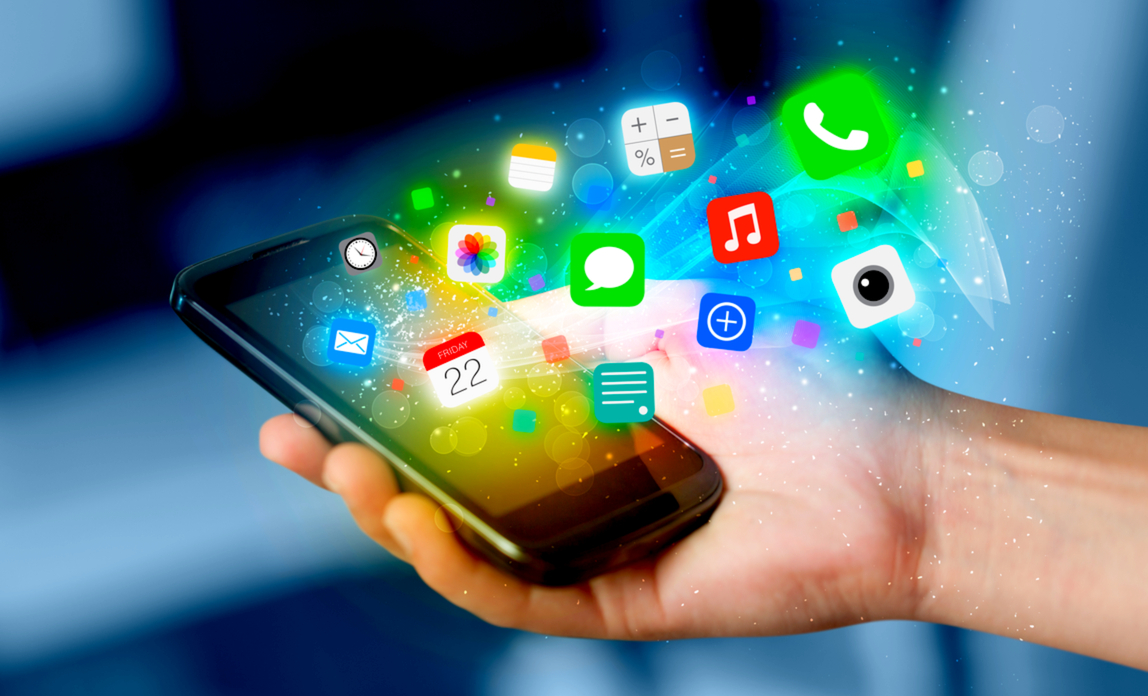
\includegraphics[width=5cm]{mobilni}\newline
     \null\hfil\hfil\makebox[5cm]{Mobilni telefon}\newline
     \vfil
     \hfil\hfil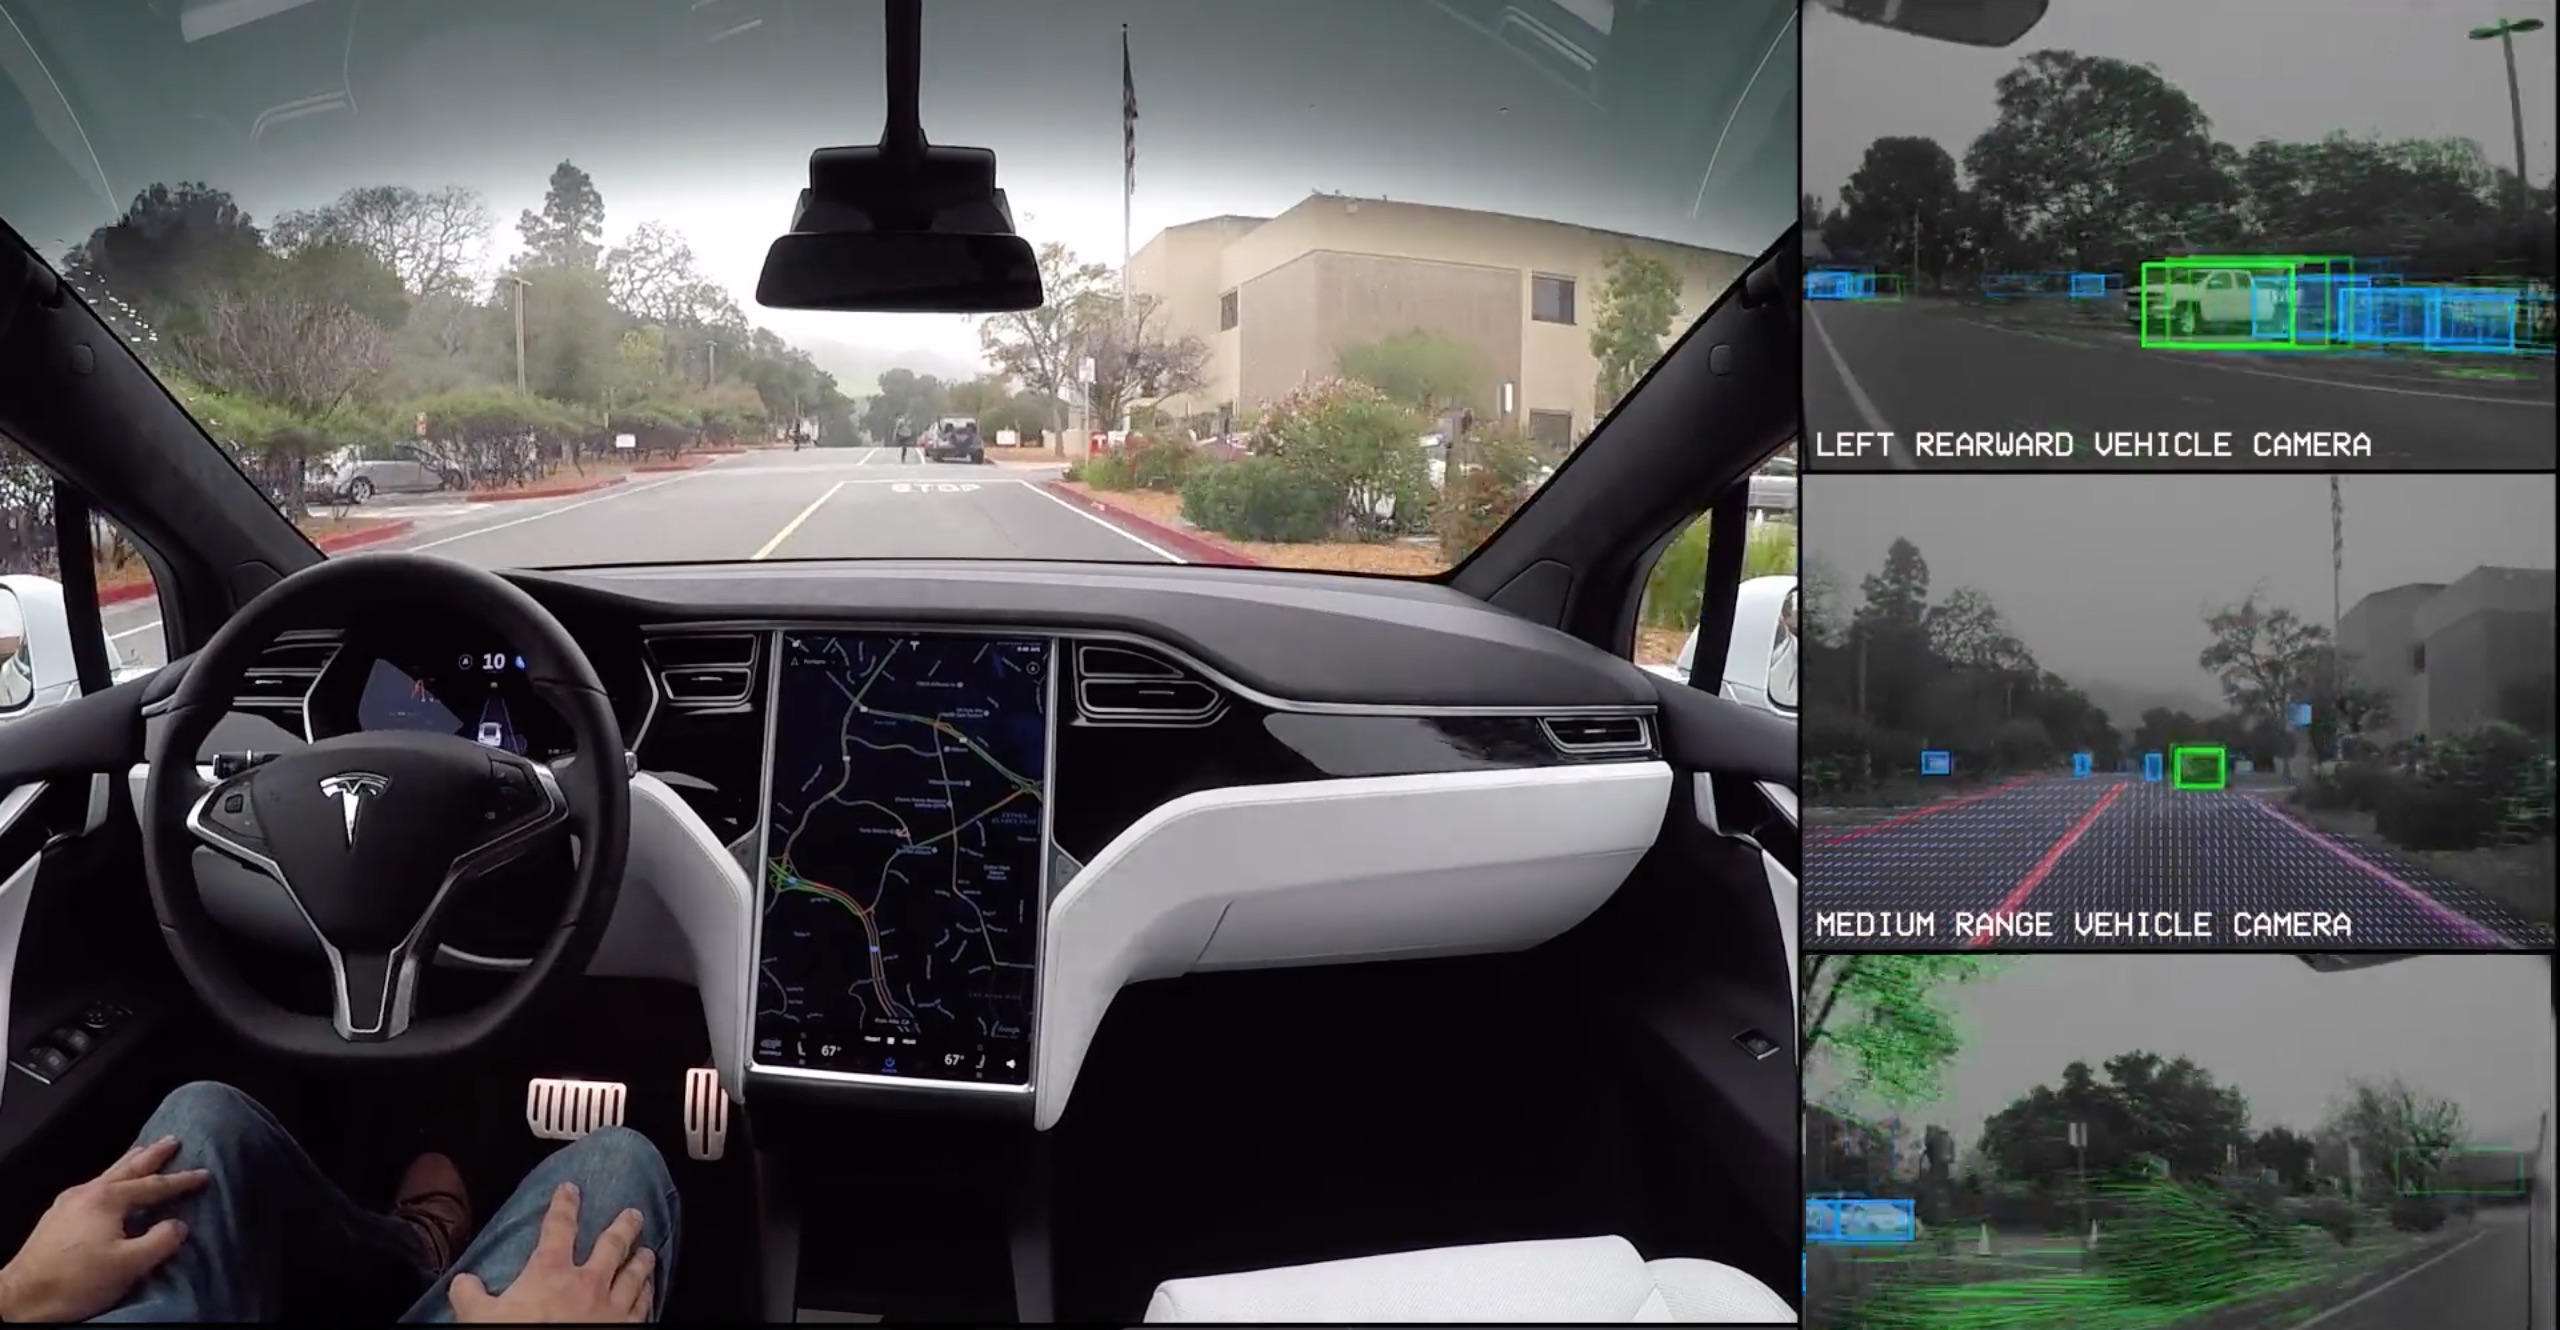
\includegraphics[width=5cm]{tesla}\hfil\hfil
       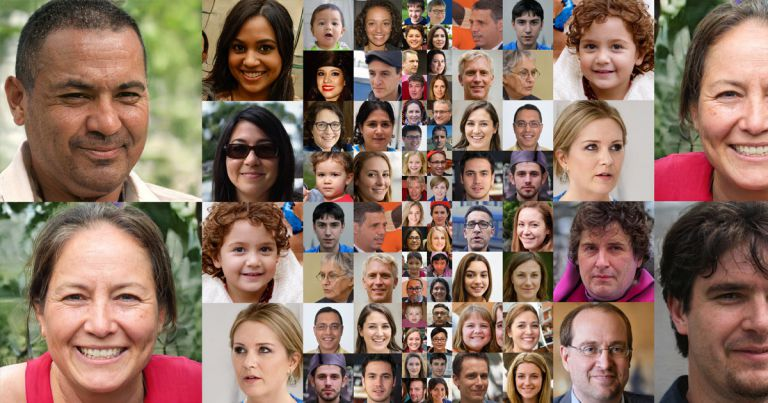
\includegraphics[width=5cm]{faces}\newline
     \null\hfil\hfil\makebox[5cm]{Tesla Autopilot}
       \hfil\hfil\makebox[5cm]{NVIDIA Neuronska Mreža}
\end{frame}

% -----------------------------------------------
%\section{Verifikacija softvera}
\begin{frame}
\frametitle{Verifikacija softvera}
\begin{itemize}
\item Specifikacija 
\item[]
\item Verifikacija 
\item[]
\item Validacija
\end{itemize}
\end{frame}


%\section{Dinamička i Statička verifikacija}
\begin{frame}
\frametitle{Dinamička i Statička verifikacija}
\begin{itemize}
\item Dinamička verifikacija
\item[]
\item Statička verifikacija
\end{itemize}

\begin{figure}

\includegraphics[width=0.5\linewidth]{engine}
\end{figure}

\end{frame}

%\section{Cilj rada}
\begin{frame}
\frametitle{Cilj rada}

\begin{itemize}
\item Da se dobije na efikasnosti u verifikaciji uz pomoć mašinskog učenja
\item[]
%\item Kreiraju se klasifikacioni modeli za određivanje da li program sadrži grešku ili ne
\end{itemize}

\end{frame}


%\section{Mašinsko učenje}
\begin{frame}
\frametitle{Mašinsko učenje}

\begin{figure}

\includegraphics[width=0.5\linewidth, height=3cm]{machine-learning}
\end{figure}

\begin{itemize}
\item Proučavanje procesa generalizacije 
\item[]
\item Konstrukcija prilagodljivih sistema sposobnih da poboljšaju svoje performanse na osnovu iskustva
\end{itemize}

\end{frame}


\begin{frame}
\frametitle{Mašinsko učenje}

\begin{itemize}
\item Nadgledano učenje
\item[]
\item Klasifikacija
\end{itemize}

\end{frame}


%\section{Eksperimentalni deo}
\begin{frame}
\frametitle{Eksperimentalni deo}

\begin{itemize}
\item Obučavanje, evaluacija i unapredjenje klasifikacionih modela, čiji je zadatak da predvide da li program sadrži grešku u kodu ili ne
\item[]
\item Implementacija programa koji na osnovu izvornog koda izračunava atribute korišćene za obučavanje modela
\item[]
\item Testiranje modela na nepoznatim programima
\end{itemize}

\end{frame}

%\section{Implementacija}
%
%  SLAJD O IZGLEDU EKSPERIMENTALNOG DELA
%
%


\begin{frame}
\frametitle{Programski jezik}

\begin{columns}[c]

\column{.45\textwidth}
\begin{itemize}
\item Python
\item[]
\item Scikit-learn
\end{itemize}

\column{.5\textwidth}
\begin{figure}

\includegraphics[width=0.6\linewidth]{python}
\end{figure}

\begin{figure}

\includegraphics[width=0.6\linewidth, height=1.5cm]{sklearn}
\end{figure}

\end{columns}

\end{frame}

\begin{frame}
\frametitle{Podaci korišćeni za obučavanje modela}

\begin{itemize}
\item Funkcije NASA-inog programa za sklapanje, transport i lansiranje svemirskih raketa i letelica
\item[]
\item 10878 objekata
\item[]
\item 1 do 3442 linije koda (prosek 42.03, medijana 23)
\end{itemize}

\end{frame}

\begin{frame}
\frametitle{Algoritmi klasifikacije}

\begin{itemize}
\item K najbližih suseda
\item[]
\item Logistička regresija
\item[]
\item Slučajne šume
\end{itemize}

\end{frame}

\begin{frame}
\frametitle{Evaluacija modela}

\begin{itemize}
%\item Standardizacija
%\item[]
\item Podela na trening i test skup
\item[]
\item K-slojna unakrsna validacija
\item[]
\item Tačnost oko 0.80
\end{itemize}

\end{frame}

\begin{frame}
\frametitle{Dodavanje novih instanci}

\begin{itemize}
\item Problem neizbalansiranih klasa
\item[]
\item Nove instance dobijene interpolacijom
\item[]
\item Tačnosti modela: 0.823 (k najbližih suseda), 0.715 (logistička regresija) i 0.848 (slučajne šume)
\item[]
\item Preciznost u slučaju klase programa sa greškom: 0,87 (slučajne šume) naspram 0,79 (k najbližih suseda).
\end{itemize}

\end{frame}

\begin{frame}
\frametitle{Izbor atributa}

\begin{itemize}
\item Kvalitetniji modeli?
\item[]
%\item NUM\_OPERATORS, NUM\_OPERANDS, LOC\_TOTAL
%\item[]
\item Tačnost, preciznost, odziv - slični kao kod modela bez izbora atributa
\end{itemize}

\end{frame}

\begin{frame}
\frametitle{Konačni model}

\begin{itemize}
\item Zasniva se na algoritmu slučajne šume
\item[]
\item Obučavan nad svim podacima
\item[]
\item Tačnost, preciznost i odziv - svi oko 0.85
\item[]
\item Poželjno je testirati model nad novim podacima
\end{itemize}

\end{frame}

\begin{frame}
\frametitle{Program koji na osnovu C koda izračunava atribute}

\begin{itemize}
\item Biblioteka pycparser 
\item[]
\item AST stablo
\item[]
\item Regularni izrazi
\end{itemize}

\end{frame}

\begin{frame}
\frametitle{Testiranje modela}

%\begin{columns}[c] 

%\column{.45\textwidth} % Left column and width
\begin{itemize}
\item Programi sa takmičenja u verifikaciji
\item[]
\item 571 program

\end{itemize}

%\column{.5\textwidth} % Right column and width
\begin{figure}
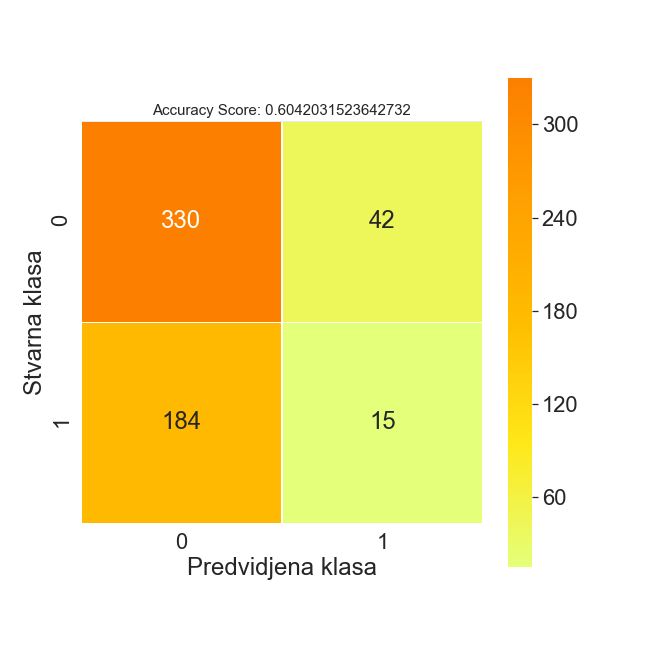
\includegraphics[width=0.5\linewidth]{confm}
\end{figure}

%\end{columns}

\end{frame}

\begin{frame}
\frametitle{Prostor za poboljšanje}

\begin{itemize}
\item Parametri modela
\item[]
\item Čitavi programi dostupni za obučavanje
\item[]
\item Druge metrike
\item[]
\item Drugi algoritmi
\item[]
\item ...
\end{itemize}

\end{frame}


\begin{frame}
\Huge{\centerline{Hvala!}}
\end{frame}

%----------------------------------------------------------------------------------------

\end{document} 